\chapter{Methodik}
\label{chapter:methodik}
In der Browser-Forensik ist eine definierte Methodik notwendig, um die Komplexität moderner Browser zu bewältigen. Sie bildet die wissenschaftliche Basis für den durchgeführten Versuch sowie einen Leitfaden für Ermittler bei zukünftigen Untersuchungen. \cite{Aggarwal.2010, Izzati.2022, Horsman.2019}	
Izzati et al. empfehlen als Vorgehensmodell für die Browser-Forensik das \textit{Generic Model Computer Forensics Investigations}, kurz \textit{GCFIM}. \cite{Yusoff.2011}
In Ihrer Anwendung auf die Browser-Forensik besteht das Modell aus vier Phasen: \cite{Izzati.2022}
\begin{itemize}
	\item \textbf{Vorbereitung:} Versuchsplanung und Konfiguration der Versuchsumgebung.
	\item \textbf{Datensammlung:} Speicherabbilder identifizieren und während des Browsing-Szenarios erstellen. 
	\item \textbf{Datenanalyse:} Suche nach Browsing-Artefakten in gesammelten Daten.
	\item \textbf{Dokumentation:} Vorgehensweise und gefundene Artefakte dokumentieren.
\end{itemize}

Die Dokumentationsphase entspricht in dieser Arbeit dem Kapitel \ref{chapter:vergleich-der-browser}, \glqq{}Vergleich der Browser\grqq{}. Die Methodik der anderen Phasen wird nachfolgend beschrieben.

\section{Vorbereitung}
\label{section:methodik-vorbereitung}
In der Vorbereitungsphase wird der durchgeführte Versuch geplant sowie die Versuchsumgebung konfiguriert. \cite{Izzati.2022} Die Versuchsplanung umfasst die Auswahl von Browsern und Tools sowie die Definition der durchzuführenden Schritte zur Kontaminierung des Rechners. Die Konfiguration der Versuchsumgebung umfasst die Installation und Konfiguration der notwendigen Software und Hardware.

\subsection{Browserauswahl}
\label{section:methodik-vorbereitung-browserauswahl}
Diese Arbeit widmet sich den zwei weit verbreiteten\footnote{Laut Statista \cite{Statista.23.05.2023}
(Stand 23. Mai 2023) sind Chrome (62,82\%), Safari (20,86\%), Edge (5,28\%) und Firefox (2,77\%) die weltweit meistgenutzten Browser. Für Safari sind nur ältere Versionen für Windows verfügbar. Microsoft Edge wurde in nur 3 von 23 untersuchten Papern untersucht, während sowohl Firefox als auch Chrome in 15 von 23 Papern analysiert wurden. \cite{Fayyad.2021, Horsman.2019, Gabet.2018, Aggarwal.2010, Oh.2011, Said.2011, Ohana.2013, Satvat.2014, Montasari.2015, Nalawade.2016, Rochmadi.2017, Md.2018, Muir.2019, Mahlous.2020, Izzati.2022}} Browsern \textit{Google Chrome} und \textit{Mozilla Firefox}.
Weiterhin werden zwei Browser mit verstärktem Schutz der Privatsphäre ausgewählt: \textit{Brave}, basierend auf Chromium, sowie der \textit{Tor-Browser}, eine modifizierte Version von Firefox.

\subsubsection*{Mozilla Firefox}
\label{subsubsection:methodik-vorbereitung-browserauswahl-firefox}
Der Browser \textit{Mozilla Firefox}, kurz \textit{Firefox}, ist ein open-source Webbrowser der gemeinnützigen Organisation Mozilla. 
Firefox hat die Funktion des \textit{Privaten Modus}. Diese ermöglicht es, ohne Speicherung von Verlaufsdaten und Cookies im Internet zu browsen.
Laut Firefox wird mit dem Privaten Modus vor dem lokalen Angreifer geschützt, wie er in \autoref{chap:theorie-angreifermodell} definiert ist, jedoch nicht vor dem Webangreifer.
Es wird ausdrücklich darauf hingewiesen, dass die besuchten Webseiten und Internetanbieter (ISP) weiterhin anhand der IP-Adresse Informationen sammeln können. \cite{Mozilla.05.06.2023}
% Für diesen Versuch: Firefox Version 112.0.2 (64 Bit)

\subsubsection*{Tor-Browser}
\label{subsubsection:methodik-vorbereitung-browserauswahl-tor}
Der \textit{Tor Browser}, kurz \textit{Tor} genannt, ist ein auf Firefox basierender Webbrowser, der das Tor-Netzwerk nutzt.
Im Gegensatz zu Firefox wird zudem mit Schutzmaßnahmen gegen den Webangreifer geworben.
Der Schutz vor dem Webangreifer ist durch das Tor-Netzwerk gegeben.
Der Tor Browser wirbt mit verstärkten Schutzmaßnahmen gegen den lokalen Angreifer. \cite{Tor.24.05.2023}

\begin{figure}[h!]
	\resizebox{\linewidth}{!}{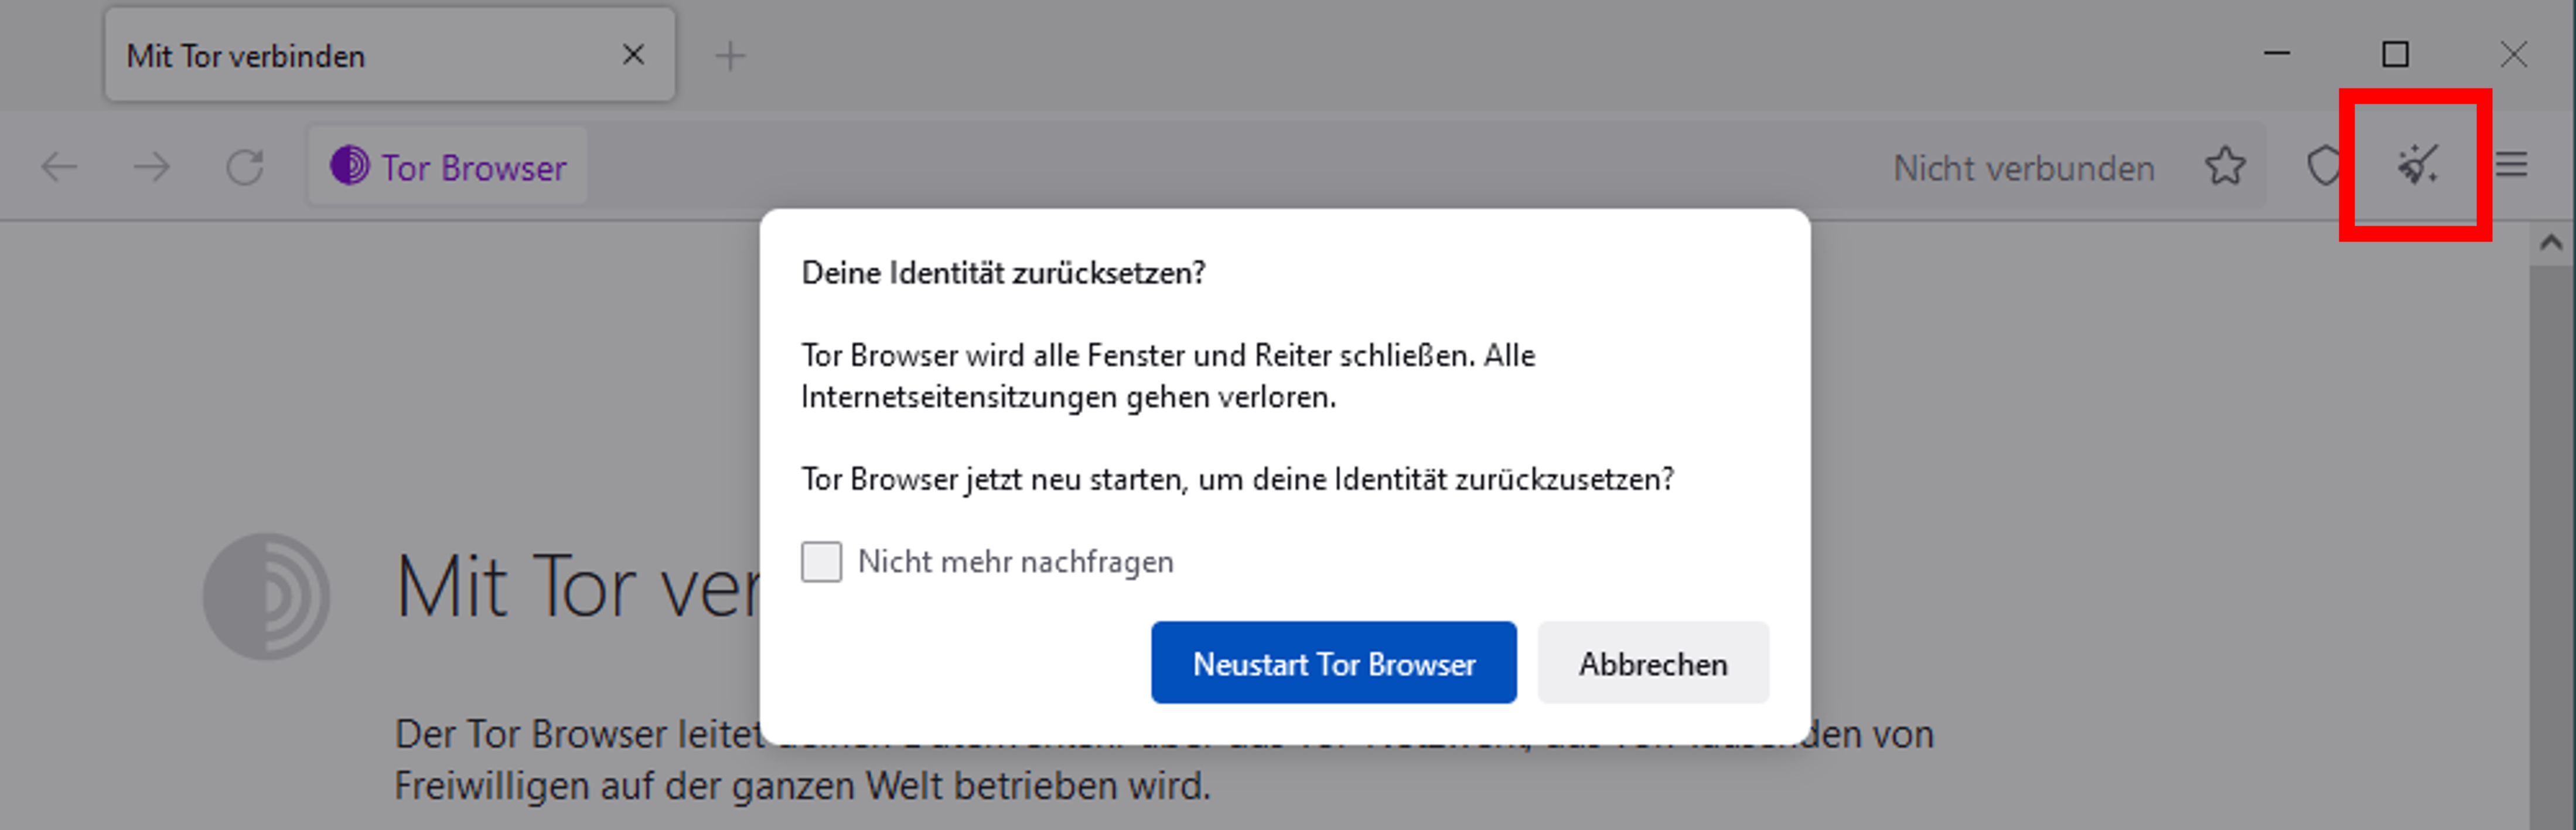
\includegraphics{bilder/tor-new-identity.png}}
	\caption{Funktion \glqq{}Neue Identität\grqq{} des Tor-Browsers}
	\label{img:tor-new-identity}
\end{figure}
Die in Abbildung \ref{img:tor-new-identity} gezeigte Funktion \glqq{}\textit{Neue Identität}\grqq{} ermöglicht es, alle aktuellen Tabs und Fenster zu schließen, sämtliche private Informationen wie Cookies und Verlauf zu löschen sowie die Verbindung mit dem Tor-Netzwerk neu zu konfigurieren. \cite{Tor.24.05.2023}
%Für diesen Versuch: Tor Version 12.0.4 (64 Bit)

\subsubsection*{Chrome}
\label{subsubsection:methodik-vorbereitung-browserauswahl-chrome}
Der von Google entwickelte \textit{Chrome} Browser bietet den \textit{Inkognitomodus} als privaten Browsing-Modus an. Laut Google werden dadurch keine Verlaufsdaten, Cookies und Websitedaten oder in Formulare eingetragene Informationen gespeichert.
Bezüglich des Schutzes vor Webangreifern macht Google keine angaben.
Chrome basiert auf dem Open-Source-Projekt \textit{Chromium}, einem freien und quelloffenen Webbrowser, der von The Chromium Projects entwickelt wird.
Dabei handelt es sich um eine von Google initiierte quelloffene Plattform für die Entwicklung von Webbrowsern.
Der Chrome Browser selbst enthält proprietäre Elemente. \cite{GoogleChrome.}

\subsubsection*{Brave}
\label{subsubsection:methodik-vorbereitung-browserauswahl-brave}
Der Open-Source-Browser \textit{Brave} wurde von Brendan Eich, dem Mitbegründer von Mozilla, mit Fokus auf Privatsphäre, Sicherheit sowie Nutzerfreundlichkeit auf Baisis des Chromium-Projekts entwickelt. 
Brave bietet Schutz vor dem lokalen Angreifer durch den \textit{Private-Window}-Modus. In diesem Modus werden laut Herstellerangaben der Browserverlauf sowie Cookies nicht lokal auf dem Gerät gespeichert. 
Um vor dem Webangreifer zu schützen, bietet Brave mit dem \textit{Private-Window-with-Tor-Connectivity}-Modus zusätzlich die Möglichkeit, eine Verbindung zum Tor-Netzwerk herzustellen. \cite{Brave.} Im Rahmen dieser Seminararbeit wird ausschließlich der Private-Window-Modus untersucht.

\subsection{Browsing-Szenario}
\label{subsection:methodik-vorbereitung-browsing-szenario}
Im Falle der transparenten Versuchsdurchführung der Browser-Forensik werden eine Reihe von Aktivitäten definiert, die für jeden untersuchten Browser durchgeführt werden -- das sogenannte \textit{Browsing-Szenario}.
In diesem Protokoll wird definiert, mit welchen Daten der Rechner kontaminiert werden soll.

Für diesen Versuch wurden ausschließlich Daten definiert, die nicht bereits vor Durchführung des Browsing-Szenarios auf dem Rechner zu finden sind. Beispielsweise sind die Zeichenketten \glqq{}twitter\grqq{} oder \glqq{}facebook\grqq{} bereits in vielen Windows-Standardanwendungen enthalten.

Folgende Schritte werden für diesen Versuch mit jedem Browser durchgeführt: 
\begin{enumerate}
\item  www.google.com aufrufen
	\begin{enumerate}[label*=\arabic*.]
	\item Alle Cookies akzeptieren (wenn gefordert)
	\item Google-Suche nach \glqq{}pfaffenhofen\grqq{}
	\end{enumerate}
\item www.google.com aufrufen
	\begin{enumerate}[label*=\arabic*.]
	\item Cookies alle akzeptieren (wenn gefordert)
	\item Google-Suche nach \glqq{}nanoradar\grqq{}
	\end{enumerate}
\item www.google.com aufrufen
	\begin{enumerate}[label*=\arabic*.]
	\item Cookies alle akzeptieren (wenn gefordert)
	\item Google-Suche nach \glqq{}mallofamerica\grqq{}
	\item Auf Suchergebnis \glqq{}mallofamerica.com\grqq{} klicken
	\end{enumerate}
\item www.google.com aufrufen
	\begin{enumerate}[label*=\arabic*.]
	\item Cookies alle akzeptieren (wenn gefordert)
	\item Google-Suche nach \glqq{}mooserliesl\grqq{}
	\item Auf Suchergebnis \glqq{}mooserliesl.de\grqq{} klicken
	\end{enumerate}
\item \glqq{}unitree.com\grqq{} über URL-Leiste öffnen
\item \glqq{}donaukurier.de\grqq{} über URL-Leiste öffnen
	\begin{enumerate}[label*=\arabic*.]
	\item Donaukurier Logo in neuem Tab öffnen
	\end{enumerate}
\item \glqq{}mail.google.com\grqq{} über URL-Leiste öffnen
	\begin{enumerate}[label*=\arabic*.]
	\item Mit google Account anmelden: 
			\begin{enumerate}[label*=\arabic*.]
			\item E-Mail = \glqq{}computerforensikvl@gmail.com\grqq{}
			\item Passwort = \glqq{}Vorlesung23!\grqq{}
			\end{enumerate}
	\item Neue E-Mail schreiben:
			\begin{enumerate}[label*=\arabic*.]
			\item Empfänger: \glqq{}cas0597@thi.de\grqq{} und \glqq{}chs3702@thi.de\grqq{}
			\item Betreff: \glqq{}Betrefftext\grqq{}
			\item Mailinhalt: \glqq{}Mailinhalt\grqq{}
			\end{enumerate}			
	\end{enumerate}
\end{enumerate}

Aus diesem Browsing-Szenario lassen sich die in Tabelle \ref{tab:pb-artefakte} dargestellten \textit{Private-Browsing-Artefakte}, kurz \textit{PB-Artefakte} ableiten. Dabei handelt es sich um Zeichenketten, die eindeutig einem Schritt im Browsing-Szenario zugeordnet werden können. Diese sind von zentraler Bedeutung in der Analysephase: Nur nach diesen Strings wird gesucht.

\begin{table}[h!]
\centering
\caption{Private-Browsing-Artefakte des Browsing-Szenarions}
\label{tab:pb-artefakte}
\begin{tabular}{|c|l|c|}
\hline
\textbf{Kategorie}           & \multicolumn{1}{c|}{\textbf{Private-Browsing-Artefakt}}                                      & \textbf{\begin{tabular}[c]{@{}c@{}}Schritt im\\  Browsing-Szenario\end{tabular}} \\ \hline
\multirow{4}{*}{Suchbegriff} & \glqq{}pfaffenhofen\grqq{}                                                                               & 1.2                                                                              \\ \cline{2-3} 
                             & \glqq{}nanoradar\grqq{}                                                                                  & 2.2                                                                              \\ \cline{2-3} 
                             & \glqq{}mallofamerica\grqq{}                                                                              & 3.2                                                                              \\ \cline{2-3} 
                             & \glqq{}mooserliesl\grqq{}                                                                                & 4.2                                                                              \\ \hline
\multirow{4}{*}{URL}         & \glqq{}mooserliesl.de\grqq{}                                                                             & 3.3                                                                              \\ \cline{2-3} 
                             & \glqq{}mallofamerica.com\grqq{}                                                                          & 4.3                                                                              \\ \cline{2-3} 
                             & \glqq{}unitree.com\grqq{}                                                                                & 5.                                                                               \\ \cline{2-3} 
                             & \glqq{}donaukurier.de\grqq{}                                                                             & 6.                                                                               \\ \hline
Bild                         & \begin{tabular}[c]{@{}l@{}}0x89 0x50 0x4E 0x47 ...\\ (PNG als Hexadezimalwerte)\end{tabular} & 6.1                                                                              \\ \hline
\multirow{4}{*}{E-Mail}      & \glqq{}computerforensikvl@gmail.com\grqq{}                                                               & 7.1.1                                                                            \\ \cline{2-3} 
                             & \glqq{}Vorlesung23! \grqq{}                                                                               & 7.1.2                                                                            \\ \cline{2-3} 
                             & \glqq{}cas0597@thi.de\grqq{}                                                                             & 7.2.1                                                                            \\ \cline{2-3} 
                             & \glqq{}chs3702@thi.de\grqq{}                                                                             & 7.2.1                                                                            \\ \hline
\end{tabular}
\end{table}


\subsection*{Konfiguration virtueller Maschinen}
\label{subsection:methodik-vorbereitung-vmkonfiguration}

Eine empfohlene Herangehensweise bei Versuchen in der Browser Forensik ist die Versuchsdurchführung in einer virtualisierten Umgebung. 
Dieser ermöglicht eine Reproduzierbarkeit und Transportierbarkeit der Ergebnisse. Pro Browser existiert eine virtuelle Maschine, kurz \textit{VM}, auf der das Browsing-Szenario durchgeführt wird. Somit werden die Versuchsumgebungen der einzelnen Browser voneinander sowie von der Analyseumgebung getrennt. \cite{Muir.2019}
Als Virtualisierungssoftware wird für diesen Versuch die kostenlose Software \textit{Oracle VM VirtualBox} verwendet. 

Alle VMs besitzen die gleiche, in Tabelle \ref{tab:vm-config} dargestellte Basiskonfiguration.
Zum Datenaustausch zwischen VM und Analyserechner wird ein \textit{gemeinsamer Ordner} eingerichtet. Somit werden beispielsweise ohne Kontaminierung der VM benötigte Programme auf dem Analyserechner heruntergeladen, in den gemeinsamen Ordner gelegt und offline auf der VM installiert.
Auf der VM werden zwei Werkzeuge der Sysinternal-Abteilung von Microsoft installiert, um in der Analysephase das Browserverhalten vollständig  untersuchen zu können: \textit{Process Monitor} ermöglicht die Aufzeichnung aller Prozessaktivitäten und \textit{Process Explorer} erweitert die Funktionen des Windows Task Managers. \cite{Markruss.05.06.2023, Markruss.05.06.2023b}
\begin{table}[h!]
\centering
\caption{Basiskonfiguration jeder VM des Versuchs}
\label{tab:vm-config}
\begin{tabular}{|l|l|}
\hline
\textbf{Betriebssystem}         & Windows 10 Pro, 64 Bit, Build: 19045.2006                                  \\ \hline
\textbf{Festplatte}             & 30 GB, VDI-Format, kein SSD Laufwerk                                       \\ \hline
\textbf{RAM}                    & 6 GB                                                                       \\ \hline
\textbf{Netzwerk}               & Netzwerkbrücke                                                             \\ \hline
\textbf{Verbindung zu Host-PC}  & Gemeinsamer Ordner                                                         \\ \hline
\textbf{Installierte Programme} & \begin{tabular}[c]{@{}l@{}}Process Monitor (Version 3.93)\\ Process Explorer (Version 17.04)\end{tabular} \\ \hline
\end{tabular}
\end{table}
Nachdem eine VM mit der Standardkonfiguration erstellt wurde, wird diese für jeden Browser dupliziert. Anschließend werden die Browser über den gemeinsamen Ordner in der entsprechenden VM installiert. Dazu wurden folgende Installationsverzeichnisse verwendet:
\begin{enumerate}
\item \textbf{Firefox}: \texttt{C:$\backslash$Program Files$\backslash$Mozilla Firefox$\backslash$firefox.exe}
\item \textbf{Tor}: \texttt{C:$\backslash$Program Files$\backslash$Tor Browser$\backslash$Browser$\backslash$firefox.exe}
\item \textbf{Chrome}: \texttt{C:$\backslash$Program Files$\backslash$BraveSoftware$\backslash$Brave-Browser$\backslash$Application$\backslash$brave.exe}
\item \textbf{Brave}: \texttt{C:$\backslash$Program Files$\backslash$Google$\backslash$Chrome$\backslash$Application$\backslash$chrome.exe}
\end{enumerate}

\subsection*{Verwendete Software}
\label{subsection:methodik-vorbereitung-verwendetesoftware}
Neben der VM Konfiguration muss die Analyseumgebung vorbereitet werden. Als Analyseumgebung dient für diesen Versuch der Rechner, auf dem die VM läuft. (Windows 10 Home, 64 Bit, Build 19045.2965)
Zur Analyse der Browser werden diverse Tools benötigt.

\subsubsection*{Autopsy}
\label{subsubsection:methodik-vorbereitung-verwendetesoftware-autopsy}
Um erstellte Festplattenabbilder zu untersuchen wird das Tool \textit{Autopsy} verwendet. Dabei handelt es sich um ein open-source Tool, das auf der Sleuthkit-Bibliothek für die forensische Analyse von Dateisystemen basiert, diese mit zusätzlichen Funktionen erweitert und eine grafische Benutzeroberfläche für die forensische Analyse bietet. \cite{Autopsy.29.03.2023} 
%Für diesen Versuch verwendet: Version 4.20.0

\subsubsection*{Volatility}
\label{subsubsection:methodik-vorbereitung-verwendetesoftware-volatility}
Um Abbilder des Arbeitsspeichers zu untersuchen wird das open-source Framework \textit{Volatility} verwendet, das speziell darauf ausgerichtet ist, Informationen und Artefakte aus dem physischen oder virtuellen Arbeitsspeicher eines Computers zu extrahieren.
%Version: Volatility3, Version 2.4.1 (aktuellster Release)
Für diesen Versuch wird \textit{Volatility3} verwendet, eine 2020 veröffentlichte vollständige Neuschreibung des Volatility Frameworks.
Volatility basiert auf Plugins, welche spezifische Funktionen und Analysen für verschiedene Aspekte des Systems bereitstellen. \cite{GitHub.05.06.2023} Für diesen Versuch werden folgende Plugins verwendet:
\begin{itemize}
\item pslist	
\item yarascan		
\item memmap	 	
\item filescan
\item svcscan
\end{itemize}
Die genaue Beschreibung der Plugins sowie deren Zusammenhang ist in der Analysephase in Abschnitt \ref{subsubsection:methodik-datenanalyse-uncommonlocations-analysemitvolatility} beschrieben.

\subsubsection*{Sonstige Tools}
\label{subsubsection:methodik-vorbereitung-verwendetesoftware-sonstigetools}
Tabelle \ref{tab:software-liste} listet zusammenfassend alle in diesem Versuch verwendeten Software-Programme, deren Verwendungszweck sowie Version auf.
Darunter befinden sich diverse zusätzliche unterstützende Tools, welche zur vollständigen Analyse benötigt werden.
\begin{table}[h!]
\centering
\caption{Vollständige Liste der verwendeten Software dieses Versuchs}
\label{tab:software-liste}
\resizebox{\linewidth}{!}{
\begin{tabular}{|l|l|l|}
\hline
\multicolumn{1}{|c|}{\textbf{Software}} & \multicolumn{1}{c|}{\textbf{Verwendungszweck}}                                              & \multicolumn{1}{c|}{\textbf{Version}} \\ \hline
Mozilla Firefox                       & Webbrowser                                                                  & 114.0.1 (64-bit) \\ \hline
Tor-Browser                       & Webbrowser                                                                  & 12.0.4 (64-bit)      \\ \hline
Google Chrome                       & Webbrowser                                                                  & 112.0.5615.138 (64-bit)    \\ \hline
Brave                       & Webbrowser                                                                  & 1.50.121 (64-bit)    \\ \hline
Windows 10 Pro                          & VM Betriebssystem                                                                & Build: 19045.2006                     \\ \hline
Process Monitor                         & Aufzeichnung Prozessaktivitäten                                                  & 3.93                                  \\ \hline
Process Explorer                        & Darstellung der Eigenschaften aktueller Prozesse                                 & 17.04                                 \\ \hline
Autopsy                                 & Analyse Festplattenabbilder                                                      & 4.20.0                                \\ \hline
Volatiltiy                              & Analyse RAM-Abbilder                                                             & Volatility3 Version 2.4.1             \\ \hline
HxD                                     & Analyse Binärdateien in hexadezimaler und ASCII-Darstellung                      & 2.5.0.0                               \\ \hline
Notepad++                               & Analyse strukturierter Dateiformate, z.B. JSON, XML                              & 8.4.5                                 \\ \hline
Registry Explorer                       & Grafische Oberfläche zur Untersuchung von Windows-Registry Hives                & 2.0.0.0                               \\ \hline
DB Browser for SQLite                   & Grafische Oberfläche zur Verwaltung und Untersuchung von SQLite-Datenbanken      & 3.12.2                                \\ \hline
sqldiff.exe                             & Befehlszeilen-Programm zur Anzeige von Unterschieden zwischen SQLite-Datenbanken & 3.42.0                                \\ \hline
ChromeCacheView                         & Einlesen von Chrome Cache-Dateien und visuelle Aufbereitung des Inhalts          & 2.46                                  \\ \hline
MZCacheView                             & Einlesen von Firefox Cache-Dateien und visuelle Aufbereitung des Inhalts         & 2.21                                  \\ \hline
FirefoxCache2                           & Erweitert MZCacheView, um Firefox \glqq{}index\grqq{}-Cachedatei zu analysieren              & Commit b50ab4f                        \\ \hline
dejsonlz4                               & Dekomprimierung von .jsonlz4-Dateien                                             & Commit c4305b8                        \\ \hline
\end{tabular}
}
\end{table}


\section{Datensammlung}
\label{section:methodik-datensammlung}
In der Phase der Datensammlung werden alle potenziellen Beweismittel identifiziert und in einem forensisch analysierbaren Format gesichert \cite{Izzati.2022}.
Im Rahmen dieser Arbeit umfasst dies die Durchführung des Browsing-Szenarios sowie das Sammeln potenzieller privater Browsing-Artefakte.

\subsection*{Process Monitor Logfiles}
\label{subsection:methodik-datensammlung-processmonitorlogfiles}
Um das Verhalten von privaten Browsingmodi möglichst vollständig zu untersuchen, schlagen Fayyad-Kazan et al. \cite{Fayyad.2021} vor, alle Aktivitäten des Browsers während Browsing-Szenarios aufzuzeichnen.
Dazu werden mit dem Tool Process Monitor alle Prozess-Aktivitäten zwischen zwei Zeitpunkten als \textit{Process Monitor Logfile} (PML) oder CSV-Datei gespeichert. \cite{Fayyad.2021, Rochmadi.2017}
Die PML-Dateien werden mithilfe des gemeinsamen Ordners auf den Analyserechner transportiert.

\subsection*{Speicherabbilder}
\label{subsection:methodik-datensammlung-speicherabbilder}
Eine der Hauptaufgaben eines Computer-Forensischen-Ermittlers ist die Erstellung und Analyse von direkten Kopien der Speichermedien des untersuchten Rechners. \cite{Hassan.2019}
Im Falle der Browser-Forensik werden Abbilder der Festplatten und des Arbeitsspeichers erstellt und analysiert.

\paragraph*{Festplatten-Image}
Da in diesem Versuch die Festplatten virtualisiert werden, wird ein Abbild aus einem sogenannten \textit{VM-Snapshot} gewonnen, eine Momentaufnahme der virtuellen Maschine. \cite{Oracle.2020} 
VM-Snapshots können \textit{aufgetaut} werden, wodurch der Zustand des Betriebssystems zum Zeitpunkt der Momentaufnahme wiederhergestellt wird.
Bei Oracle VM VirtualBox kann ein VM Snapshot über die grafische Oberfläche erstellt werden.
Durch den Snapshot wird ein \textit{Virtual Disk Image}, eine VDI-Datei, im Snapshot-Ordner der VM erzeugt. Diese Laufwerksdatei enthält nur differentielle Daten zum vorherigen Snapshot.
Um aus den differentiellen Daten ein vollständiges Festplatten-Image zu erzeugen, muss ein \textit{vollständiger Klon} des Snapshots erstellt werden. Die VDI-Datei der geklonten VM entspricht einem vollständigem Abbild der Festplatte zum Zeitpunkt des durchgeführten Snapshots.

Da Autopsy nicht das VDI-Format unterstützt, müssen die Laufwerksdateien der geklonten Snapshots in das generische \textit{Image}-Format (.img) umgewandelt werden.
Durch Nutzung des VirtualBox Befehlszeilen-Tool \textit{vboxmanage} wird mit dem Befehl \texttt{vboxmanage clonehd <VDI\_File>.vdi <IMG\_File>.img --format raw} die VDI-Datei ein eine IMG-Datei umgewandelt.
Um ein Festplatten-Image in Autopsy einzulesen, wird ein neuer \textit{Fall} (engl. Case) erstellt. Das Einlesen eines ca. 30 GB großen Festplatten-Images dauerte mit allen aktivierten Autopsy-Plugins zwischen 5 und 7 Stunden.

\paragraph*{RAM-Dump}
Ein \textit{RAM-Dump} erfasst den Zustand des Arbeitsspeichers, einschließlich der im Speicher befindlichen Daten, Programme und Prozesse zu einem bestimmten Zeitpunkt \cite{TILT.25.03.2023}.
VirtualBox empfiehlt, Abbilder des RAMs ebenfalls über das vboxmanage Befehlszeilen-Tool durchzuführen.
Im Unterschied zu Festplatten-Images können RAM-Dumps nur im angeschalteten Zustand der virtellen Maschine mithilfe des Befehls \texttt{vboxmanage debugvm <VM Name> dumpvmcore --filename <RAM Dump Dateiname>.elf} durchgeführt werden. RAM-Dumps im .elf Format können direkt vom Analysetool Volatility innerhalb weniger Minuten eingelesen werden.		

\paragraph*{Zeitpunkte zur Datensammlung}
Wichtig für die Qualität der Versuchsergebnisse sind die Zeitpunkte während des Browsing-Szenarios zum Sammeln der Daten.
In der Literatur wählen die Autoren meist ohne Begründung Zeitpunkte zur Datensammlung \cite{Sajan.2021, Nalawade.2016, Montasari.2015, Satvat.2014, Said.2011, Aggarwal.2010}.
Dieses Problem haben Muir, Leimich und Buchanan erkannt und spezifische Zeitpunkte zur Datensammlung vorgeschlagen. Diese ermögliche eine vollständige Analyse des Browserverhaltens vor, während und nach dem Browsing-Szenario. \cite{Muir.2019}. Wie in Abbildung \ref{img:zeitpunkte-datensammlung} dargestellt, wurde sich an diesen Zeitpunkten für diesen Versuch orientiert.
\begin{figure}[h!]
	\centering
	\small
	\centerline{\resizebox{\linewidth}{!}{\input{bilder/datensammlung-zeitpunkte-tor-Latex.pdf_tex}}}
	\caption{Zeitpunkte zur Datensammlung während der Versuchsdurchführung nach \cite{Muir.2019}}
	\label{img:zeitpunkte-datensammlung}
\end{figure}

Der erste RAM-Dump sowie der erste VM-Snapshot nach der Browser-Installation, vor Beginn des Browsing-Szenarios, dienen als Baseline für die Analyse, da in diesen Speicherabbildern kein PB-Artefakt gefunden werden darf.
Nachdem der private Modus im Browser geöffnet wird und bevor das Browsing-Szenario beginnt, wird die Aufnahme des ersten Process Monitor Logfiles gestartet. Um ausschließlich Schreiboperationen aufzuzeichnen, die auf das private Browsing zurückzuführen sind, wird die Aufzeichnung erst nach dem erstmaligen Öffnen des Browsers im privaten Modus gestartet.
Nach Durchführung des Browsing-Szenarios, während der Browser noch geöffnet ist, wird die Aufnahme des ersten Process Monitor Logfiles gestoppt. Weiterhin wird ein zweiter RAM-Dump sowie VM-Snapshot erstellt. Anschließend wird eine zweite Process Monitor Aufzeichnung gestartet. 
Nachdem der Browser geschlossen wurde, wird die Aufzeichnung des zweiten Process Monitor Logfiles beendet. Somit enthält das zweite Logfile alle Prozessaktivitäten vom Schließen der Browsers. Zusätzlich wird ein dritter RAM-Dump sowie  VM-Snapshot erstellt. 
Nach Herunterfahren der VM wird ein vierter VM-Snapshot erstellt.

\paragraph*{Sonderfälle}
Dieses Vorgehen zur Datensammlung wird bei allen Browsern durchgeführt. Einzig der Tor-Browser weicht davon ab. Um die \glqq{}Neue Identität\grqq{}-Funktion des Tor-Browsers zu berücksichten, werden zusätzlich Daten vor und nach der Erstellung einer \glqq{}Neuen Identiät\grqq{} gesammelt. Wie in Abbildung \ref{img:zeitpunkte-datensammlung-tor} dargestellt, umfasst dies einen zusätzlichen RAM-Dump sowie VM-Snapshot und ein weiteres Process Monitor Logfile.
\begin{figure}[h!]
	\centering
	\small
	\centerline{\resizebox{\linewidth}{!}{\input{bilder/datensammlung-zeitpunkte-Latex.pdf_tex}}}
	\caption{Zeitpunkte zur Datensammlung während der Versuchsdurchführung für den Tor-Browser}
	\label{img:zeitpunkte-datensammlung-tor}
\end{figure}

Bei Durchführung des Browsing-Szenarios für den Firefox-Browser wurde nach erstmaligem Öffnen des Browsers automatisch die Firefox Datenschutz-Webseite \texttt{https://www.mozilla.org/\\
de/privacy/firefox/} im nicht-privaten Modus durch den Browser geöffnet. 

Sowohl Google Chrome als auch der Brave Browser öffneten sich automatisch nach der abgeschlossenen Installation im nicht-privaten Modus.

\section{Datenanalyse}
\label{section:methodik-datenanalyse}
Nachdem die Daten in Form von Process Monitor Logfiles und Festplatten- sowie RAM-Speicherabbildern gesammelt wurden, wird nach den PB-Artefakten aus Tabelle \ref{tab:pb-artefakte} in Abschnitt \ref{subsection:methodik-vorbereitung-browsing-szenario} gesucht. 
Die gesammelten Daten des Versuchs werden zur Vereinfachung der Analyse in drei Kategorien aufgeteilt: \textit{Common Locations}, \textit{Uncommon Locations} sowie \textit{Registry}.

\subsection{Common Locations}
\label{subsection:methodik-datenanalyse-commonlocations}
Die sogenannten \textit{Common Locations} beziehen sich im Zusammenhang der Browser-Forensik auf die standardmäßigen Verzeichnisse eines Browsers auf der Festplatte, beispielsweise Ordner von Browsern zur Verwaltung von Nutzerdaten.
Untersucht werden Common Locations mittels \textit{Whitebox-Analyse}. Dabei besitzt der Forensiker Fachwissen über das Browserverhalten. Anhand dieses Wissens können gezielt potenzielle Beweise gesammelt werden. \cite{Bonetti.2014}

Bei diesem Versuch werden die Speicherorte über die Schreiboperationen der Process Monitor Logfiles identifiziert.
Anschließend wird für jede Datei in den Speicherorten geprüft, ob PB-Artefakte enthalten sind.
Dazu sind zwei Schritte notwendig:
\begin{enumerate}
\item \textbf{Dateiextraktion}: Extrakion der Datei aus dem Speicherabbild. Wenn die Datei nicht mehr vorhanden ist, werden dazu ggf. Tools zur Dateiwiederherstellung benötigt.
\item \textbf{Dateianalyse}: Um zu überprüfen ob die Datei PB-Artefakte enthält, werden ggf. Tools für spezielle Dateiformate benötigt, beispielsweise Dekomprimierungstools.
\end{enumerate}

\paragraph*{Identifikation der Common Locations}
Um die gängigen Browserpfade und -dateien zu identifizieren, werden die in den Process Monitor Logfiles aufgezeichneten Datei-Schreibaktivitäten der Browserprozesse ausgewertet.

Dazu wird jedes Logfile mit dem Process Monitor eingelesen. Anschließend werden die Aktivitäten gefiltert. Wie in Abbildung \ref{img:procmon-writefile-filter} dargestellt, wird dazu ausschließlich die Option \glqq{}File System Activity\grqq{} ausgewählt.
\begin{figure}[h!]
	\centerline{\resizebox{0.7\linewidth}{!}{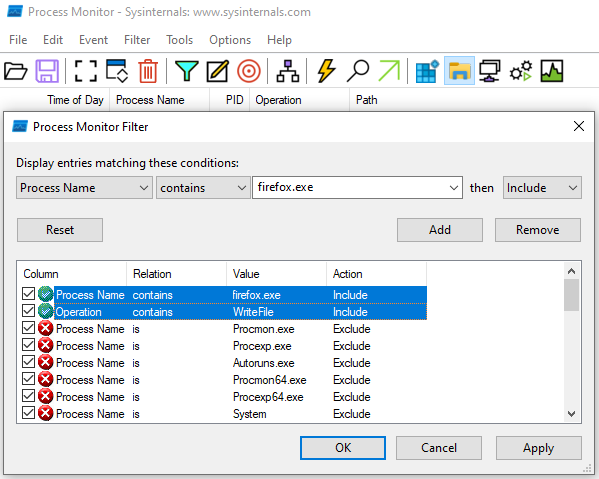
\includegraphics{bilder/process-monitor-filter.png}}}
	\caption{Process Monitor Filter für Datei-Schreiboperationen}
	\label{img:procmon-writefile-filter}
\end{figure}

Anschließend wird als Prozessname der Browserprozess gesetzt:
\begin{itemize}
\item \textbf{Firefox}: firefox.exe
\item \textbf{Tor-Browser}: firefox.exe und tor.exe
\item \textbf{Chrome}: chrome.exe
\item \textbf{Brave}: brave.exe
\end{itemize}
Da PB-Artefakte nur über Schreiboperationen entstehen können, wird als Prozessoperation \glqq{}WriteFile\grqq{} gesetzt.
Die gefilterte Logfile wird als CSV exportiert, um sie dann in Excel zu öffnen und irrelevante Spalten sowie Duplikate zu löschen.
Die geschriebenen Dateien werden anschließend browserspezifisch gruppiert.

\paragraph*{Prüfung auf PB-Artefakte}
Nachdem die geschriebenen Browserdateien identifiziert und gruppiert wurden, wird für jede Datei geprüft, ob PB-Artefakte enthalten sind. Folgende, in Abbildung \ref{img:dateiextraktion-und-analyse} dargestellte Schritte sind zur Dateiextraktion und Dateianalyse notwendig:
Die Datei befindet sich entweder im entsprechenden Festplatten-Image oder ist im RAM-Dump. 
Wenn die Datei nicht mit Autopsy aus dem Festplatten-Image extrahiert werden kann und sich der Dateiname in der Ausgabe des Volatiltiy Plugins \textit{filescan} (\texttt{vol.py -f ram\_dump.elf windows.filescan > filescan.txt}) befindet, wird diese mit dem Volatility Plugin \textit{dumpfiles} (\texttt{vol.py -f ram\_dump.elf -o $\backslash$some\_folder$\backslash$ windows.dumpfiles --virtaddr <virtual file address>}) aus dem RAM extrahiert.
Wenn auch dies nicht möglich ist und es sich um eine temporäre Datei (.tmp) handelt, wird versucht die enstprechende nicht-temporäre Datei zu extrahieren. 
Im Falle der Datei \glqq{}some-file.json.tmp\grqq{} wird beispielsweise geprüft, ob die Datei \glqq{}some-file.json\grqq{} existiert.
Nachdem die Datei extrahiert wurde und ggf. mit einem Tool zu Analyse vorberarbeitet wurde, wird geprüft, ob die Datei PB-Artefakte enthält.
\begin{figure}[h!]
	\centering
	\small
	\centerline{\resizebox{\linewidth}{!}{\input{bilder/process_monitor_to_excel-Latex.pdf_tex}}}
	\caption{Vorgehen zur Dateiextration und -analyse}
	\label{img:dateiextraktion-und-analyse}
\end{figure}

\paragraph*{SQLite-Datenbanken}
\label{subsubsection:methodik-datenanalyse-commonlocations-sqlitedbs}
Eine besondere Rolle unter den Common Locations bei Browsern nehmen SQLite-Datenbanken ein. 
Sie speichern und verwalten Nutzerinformationen, wie Lesezeichen, Browserverlauf, Caches, Cookies in Datenbankdateien, ohne einen separaten Datenbankserver zu benötigen.

Wie in Abbildung \ref{img:dateiextraktion-und-analyse-sqlite} dargestellt, erfolgt die Dateiextraktion analog zur Vorgehensweise bei den Datei-Schreiboperationen der Process Monitor Logfiles. Um die SQLite-Datenbanken zu analysieren wird jede Datenbank mit der gleichen Datenbank aus dem vorherigen Snapshot mithilfe des Befehlszeilentools \textit{sqldiff.exe} (\texttt{sqldiff.exe database1.sqlite database2.sqlite}) verglichen. Die Inhaltsunterschiede werden für jede SQLite-Datei in jedem Snapshot untersucht und in einer Excel Tabelle festgehalten.
Datenbankänderungen einer SQLite-Datei werden zuerst im \textit{Write-Ahead Log}, kurz \textit{WAL}, vorübergehend protokolliert. 
Um potenzielle PB-Artefakte zu berücksichtigen, wird der WAL mithilfe der sqlite3 Befehlszeile (\texttt{sqlite3> PRAGMA wal\_checkpoint;}) in die SQLite-Hauptdatenbank geschrieben.
\begin{figure}[h!]
	\centering
	\small
	\centerline{\resizebox{\linewidth}{!}{\input{bilder/sqlite-methodology-Latex.pdf_tex}}}
	\caption{Vorgehen zur Dateiextraktion und -analyse von SQLite-Datenbanken}
	\label{img:dateiextraktion-und-analyse-sqlite}
\end{figure}

\subsection{Uncommon Locations}
\label{subsection:methodik-datenanalyse-uncommonlocations}
\textit{Uncommon Locations} beziehen sich auf Verzeichnisse, die nicht zu den gängigen Speicherorten gehören. 
Bei Festplatten-Images handelt es sich dabei meist um Dateien des Betriebssystems\footnote{
In der betrachteten Literatur wird die sogenannte \textit{pagefile.sys} als Teil der Uncommon Locations unter Windows untersucht. Diese Datei wird verwendet, um Daten aus dem Hauptspeicher auf die Festplatte auszulagern, wenn der verfügbare physische Speicher begrenzt ist. \cite{MicrosoftLearn.21.03.2023}
In der betrachteten Literatur wurde nur die Stringsuche im Hexadezimaleditor als Analysemethode identifiziert. Wie in diesem Abschnitt beschrieben, ist dies aufgrund der fehlenden Zuordnung zu einem spezifischen Browser unzureichend. Um eine Beweisauthentifizierung gemäß dem Ziel der Arbeit zu garantieren, wird der Inhalt der \textit{pagefile.sys} nicht untersucht. Gleiches gilt für die Speicherverwaltungsdatei \textit{hiberfile.sys}
} oder andere Festplattenbereiche, wie beispielsweise unallokierte Speicherbereiche oder der Arbeitsspeicher.
Uncommon Locations werden ohne Vorwissen über das Browserverhalten sowie ohne Vorverarbeitung der Dateien mithilfe der \textit{Blackbox-Analyse} untersucht:
Im Kontext der Browser Forensik werden dazu Stringsuchen nach PB-Artefakten über die gesamten Speicherabbilder durchgeführt.
Dies ist nur mit Unterstützung durch Forensik-Tools möglich. \cite{Bonetti.2014} Somit wird bei der Analyse der Uncommon Locations auf die Vollständigkeit der Tools vertraut.

\subsubsection*{Analyse mit Autopsy}
\label{subsubsection:methodik-datenanalyse-uncommonlocations-analysemitautopsy}
Bei den Uncommon Locations wird Autopsy als forensisches Werkzeug zur Analyse der Festplatten-Images verwendet.
Dazu wird eine Stichwortsuche mit den in Tabelle \ref{tab:pb-artefakte} definierten PB-Artefakten über das gesamte eingelesene Festplatten-Image durchgeführt.
Autopsy bietet dazu die in Abbildung \ref{img:autopsy-keywordsuche} dargestellte Funktion zur Suche nach Strings, Teilstrings oder regulären Ausdrücken in Dateinamen und Dateiinhalten an.
\begin{figure}[h!]
	\centerline{\resizebox{0.85\linewidth}{!}{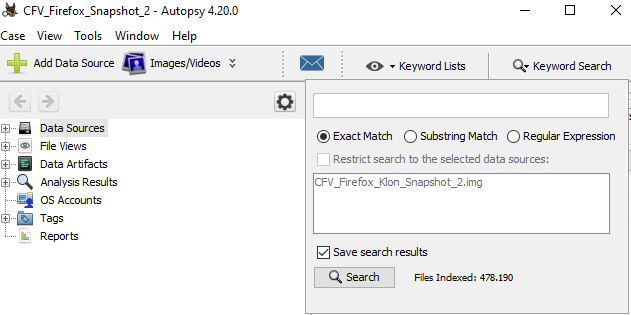
\includegraphics{bilder/autopsy-search.png}}}
	\caption{Autopsy Funktion zur Stichwortsuche}
	\label{img:autopsy-keywordsuche}
\end{figure}

Zusätzlich kategorisiert Autopsy automatisch die Dateien eines Festplatten-Images. Für diesen Versuch sind folgende Dateikategorien von Interesse:
\begin{itemize}
\item Web Bookmarks
\item Web Cookies
\item Web History
\item Web Categories
\end{itemize}

\subsubsection*{Analyse mit Volatility}
\label{subsubsection:methodik-datenanalyse-uncommonlocations-analysemitvolatility}
Bei der Analyse des Arbeitsspeichers als Uncommon Location ist es von entscheidender Bedeutung, dass ein gefundener String eindeutig einem Browserprozess zugeordnet werden kann. 

In der Literatur werden Arbeitsspeicherabbilder oft unzureichend durch eine Stichwortsuche im Hexadezimaleditor analysiert. \cite{Rochmadi.2017, Md.2018, Montasari.2015}
Dies kann aber nach Auffassung der Autoren dieser Arbeit zu Fehlschlüssen führen. Beispielhaft wird dies in Abbildung \ref{img:textfile-ram-artifact} gezeigt: Ein String, der in einer Textdatei auf dem Desktop gespeichert ist, wird im Hexadezimaleditor HxD angezeigt, obwohl kein Browsing-Szenario durchgeführt wurde.
\begin{figure}[h!]
	\centering
	\subcaptionbox{String in Textdatei}{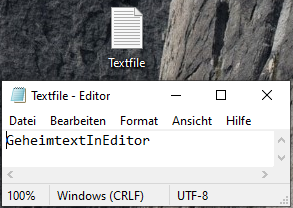
\includegraphics[width=0.30\textwidth]{bilder/ram-editor1.png}}%
	\hfill
	\subcaptionbox{String als Hexadezimalwert in RAM-Dump (geöffnet mit HxD)}{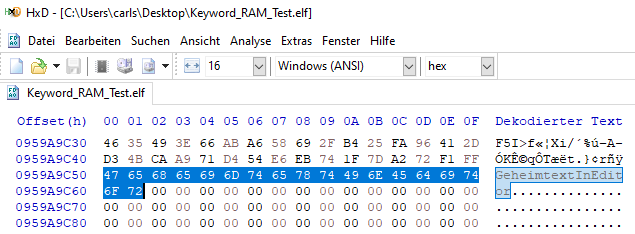
\includegraphics[width=0.65\textwidth]{bilder/ram-editor2.png}}%
	\caption{Beispiel für ein RAM-Artefakt ohne vorheriges Browsing-Szenario}
	\label{img:textfile-ram-artifact}  
\end{figure}

Um einen im RAM gefundenen String einem Browserprozess zuordnen zu können, wird deshalb das forensiche Analysetool Volatility mit dem Plugin \textit{Yarascan} verwendet.
Mithilfe sogenannter \textit{Yara-Regeln} (engl. Yararules) wird nach bestimmten Mustern im Arbeitsspeicher gesucht.
Die für diesen Versuch verwendeten Yara-Regeln entsprechen den Strings der PB-Artefakte in Tabelle \ref{tab:pb-artefakte}. Zusätzlich sucht eine Regel nach HTML-Fragmenten, die eindeutig einer besuchten Seite des Browsing-Szenarios zuzuordnen sind. \cite{Said.2011}
Alle verwendeten Yara-Regeln sind im Anhang \ref{appendix:yara-regeln} aufgelistet.
Um den RAM-Dump nach den Yara-Regeln zu durchsuchen, wird folgender Befehl ausgeführt: \texttt{vol.py -f ram\_dump.img windows.vadyarascan --yara-file yara\_rules.yara > yarascan.txt}
Nachdem der RAM-Dump nach den Regeln durchsucht wurde, gibt die Yarascan-Ausgabe für jeden gefundenen String die PID des Prozesses, in dem der String gefunden wurde, sowie die virtuelle Speicheradresse des gefundenen Strings an.

\begin{figure}[h!]
	\centering
	\small
	\centerline{\resizebox{\linewidth}{!}{\input{bilder/yarascan_plugin_tree-Latex.pdf_tex}}}
	\caption{Abhängigkeiten der verwendeten Volatility-Plugins yarascan, pslist und memmap}
	\label{img:volatility-plugins}
\end{figure}

Wie in Abbildung \ref{img:volatility-plugins} dargestellt, wird davon ausgehend mit dem Plugin \textit{pslist} (\texttt{vol.py -f ram\_dump.img windows.pslist --pid <PID> > pslist.txt}) der Prozessname der PID ermittelt, in dem der String gefunden wurde.

Oft ist bei einem gefundenen String von Interesse, ob in den Speicheradressen vor und nach dem Treffer weitere Zusammenhänge erkennbar sind.
Mithilfe des Plugins \textit{memmap} (\texttt{vol.py -f ram\_dump.img windows.memmap --pid <PID> > memmap.txt}) wird die Abbildung der virtuellen Speicheradressen eines Prozesses auf die Byte-Offsets der extrahierten Speicherseite des Prozesses ermittelt.
Diese Seite kann mithilfe des \glqq{}dump\grqq{}-Flags extrahiert werden: \texttt{vol.py -f ram\_dump.img -o $\backslash$dump\_dir$\backslash$ windows.memmap --pid <PID> -{}-dump}.
In einem Hexadezimaleditor, wie HxD, kann die Umgebung des String-Treffers anhand des ermittelten Byte-Offsets in der Speicherseite untersucht werden.

\subsection{Registry}
\label{subsection:methodik-datenanalyse-registry}
Die letzte Kategorie analysierter Daten umfasst die Artefakte der Registry.
Diese zählen sowohl zu den Common als auch Uncommon Locations und werden deshalb als eigene Kategorie aufgeführt.

\paragraph*{Common Locations}
%*** TODO: Common location: Shellactivities Key ***
%	existiert nicht mehr --> Nicht mehr vorhanden in aktueller Version (Verweis auf E-Mail)
Als Teil der Common Locations werden die Registry-Aktivitäten in den Process Monitor Logfiles analysiert.
\begin{figure}[h!]
	\centerline{\resizebox{0.7\linewidth}{!}{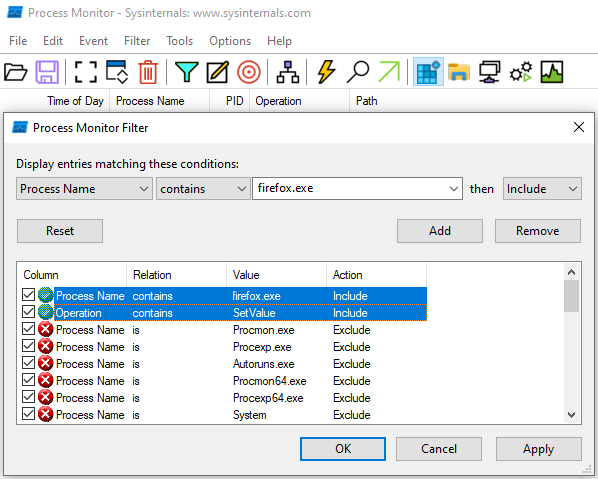
\includegraphics{bilder/process-monitor-filter-registry.png}}}
	\caption{Process Monitor Filter für Registry-Schreiboperationen}
	\label{img:procmon-setvalue-filter}
\end{figure}
Wie in Abbildung \ref{img:procmon-setvalue-filter} gezeigt, wird zunächst das Logfile nach \glqq{}Registry Activity\grqq{} sowie Einträgen mit der Operation \glqq{}SetValue\grqq{} sowie dem Browser-Prozessnamen gefiltert.
Als CSV-Datei wird das Logfile in Excel weiter verarbeitet, indem Duplikate gelöscht werden und die geschriebenen Registry-Keys browserspezifisch gruppiert werden.
	
\paragraph*{Uncommon Locations}
Unter Betrachtung als Uncommon Location werden alle Windows Registry Hives in jedem Festplatten-Image mit dem Registry Explorer untersucht.
Dabei wird zwischen Hives zur Speicherung von Systemeinstellungen (System-Hives) und individuellen Benutzerkonfigurationen (User-Hives) unterschieden. Diese in Tabelle \ref{tab:windows-Registry Hives} dargestellten Hives werden von Windows beim Start geladen und dienen Systemkomponenten und Anwendungen als Quelle für Einstellungen und Informationen. \cite{Haircutfish.04.11.2022}
Zur Analyse wird jeder Hive aus den Fesplatten-Images extrahiert und in eine Registry-Explorer-Sitzung geladen, um eine Stringsuche nach PB-Artefakten durchzuführen.

\begin{table}[h!]
\centering
\caption{Windows Registry Hives}
\label{tab:windows-Registry Hives}
\resizebox{\linewidth}{!}{
\begin{tabular}{lllll}
\cline{1-2}
\multicolumn{2}{|c|}{\textbf{System-Hives (C:\textbackslash{}Windows\textbackslash{}System32\textbackslash{}Config)}} &  &  &  \\ \cline{1-2}
\multicolumn{1}{|l|}{\textbf{Dateiname}}             & \multicolumn{1}{l|}{\textbf{Inhalt}}                                                                           &  &  &  \\ \cline{1-2}
\multicolumn{1}{|l|}{\textit{DEFAULT}}               & \multicolumn{1}{l|}{Standardkonfigurationseinstellungen für neue Benutzerprofile}                             &  &  &  \\ \cline{1-2}
\multicolumn{1}{|l|}{\textit{SAM}}                   & \multicolumn{1}{l|}{Sicherheitskontendaten, einschließlich der Benutzerkonten und deren Kennwörter}          &  &  &  \\ \cline{1-2}
\multicolumn{1}{|l|}{\textit{SECURITY}}              & \multicolumn{1}{l|}{Sicherheitsinformationen für die Zugriffssteuerung und Authentifizierung}                 &  &  &  \\ \cline{1-2}
\multicolumn{1}{|l|}{\textit{SOFTWARE}}              & \multicolumn{1}{l|}{Konfigurationsdaten für installierte Software und Anwendungen}                            &  &  &  \\ \cline{1-2}
\multicolumn{1}{|l|}{\textit{SYSTEM}}                & \multicolumn{1}{l|}{Systemkonfigurationseinstellungen und Gerätetreiberinformationen}                         &  &  &  \\ \cline{1-2}
                                                     &                                                                                                                &  &  &  \\ \cline{1-2}
\multicolumn{2}{|c|}{\textbf{User-Hives (C:\textbackslash{}Users\textbackslash{}\textless{}username\textgreater{})}}                  &  &  &  \\ \cline{1-2}
\multicolumn{1}{|l|}{\textbf{Dateiname}}             & \multicolumn{1}{l|}{\textbf{Inhalt}}                                                                           &  &  &  \\ \cline{1-2}
\multicolumn{1}{|l|}{\textit{NTUSER.DAT}}            & \multicolumn{1}{l|}{Individuelle Einstellungen und Konfigurationen für den angemeldeten Benutzer}              &  &  &  \\ \cline{1-2}
\multicolumn{1}{|l|}{\textit{USRCLASS.DAT}}          & \multicolumn{1}{l|}{Dateizuordnungen und Registrierungseinstellungen für den angemeldeten Benutzer}            &  &  &  \\ \cline{1-2}
\end{tabular}
}
\end{table}
	

